\chapter{Diseases of Attitude}

In this opening lecture Jim Rohn proceeds less by formal proof than by a disciplined sequence of maxims, comparisons, and worked contrasts. We can still write the chapter in a mathematically serious register if we keep the source honest: first the negative is admitted as a normal feature of life, then inactivity is shown to have defaults, then the lecture narrows into a visible list of diseases, and finally the whole discussion is gathered into a simple causal model of thought, input, and outcome.

\section{Negative Is Normal, But It Must Be Handled}

The lecture begins by removing a false embarrassment. We are not to study the negative because it is glamorous, but because it is ordinary. The weeds metaphor matters here: weeds are not a scandal in a garden; they are part of the standing conditions under which a garden exists.

\begin{equation}
\text{Negative} = \text{normal}, \qquad \text{Negative} \neq \text{successful}.
\end{equation}

That distinction is the lecture's first clean move. Once the negative is admitted as normal, the operative verb changes. We are not asked to love it, and we are not permitted to deny it; we are asked to handle it. This is also where Rohn insists that the listener should be a student rather than a follower. The point is not blind agreement, but disciplined recognition: if we pretend there are no weeds, the weeds still take the garden.

\section{The War Frame, Default Rules, And Activity}

From that initial classification the lecture broadens into a war frame. The broadening is not decorative. It is the mechanism by which passivity stops looking harmless. If good is inactive, something else does not remain politely absent; it moves in.

\begin{align}
\neg \text{light} &\Rightarrow \text{darkness},\\
\neg \text{active good} &\Rightarrow \text{evil},\\
\text{sleeping democracy} &\Rightarrow \text{tyranny}.
\end{align}

These are lecture rules rather than mathematical theorems, but they do the work of rules. They identify the defaults. The world has drift built into it. Left alone, it does not hold the good in place.

Rohn immediately adds the balancing proposition. Evil is no match for good, but only on the condition that good is active. The garden metaphor now becomes sharper.

\begin{equation}
\text{human activity} > \text{weeds}, \qquad \text{provided activity is present}.
\end{equation}

That is why the lecture next translates the war frame into a small quantitative discipline:

\begin{equation}
\text{labor}:\text{rest} = 6:1.
\end{equation}

The lecturer's gloss is more severe than the proverb as it is usually heard. The hidden message is not merely that one day of rest is allowed. It is that one day of rest is enough. Too much ease gives too much room to the counter-force.

\begin{equation}
\text{enterprise} > \text{ease}, \qquad \text{activity} > \text{drift}.
\end{equation}

\paragraph{A worked heuristic.}
The internal derivation is short and worth preserving.
\begin{enumerate}
\item The negative is part of the environment.
\item Therefore passivity is not neutral.
\item Hence the problem is not whether we rest, but how much ground we yield while resting.
\item The ratio \(6:1\) becomes a discipline of activity.
\item The jungle metaphor then follows naturally: if we rest too long, the village is overtaken.
\end{enumerate}

The retirement remark belongs to this same logic. It is intentionally overstated, but structurally it serves to keep the warning sharp: disengagement can become surrender.

\section{From War To Diagnosis: The List Begins}

At this point the lecture deliberately narrows. After recapping the war and the weeds, Rohn turns from global frame to local diagnosis: let us make a list of the diseases of attitude that wreck a life. The tonal shift matters. We are no longer speaking in pairs of abstractions only; we are now naming the points at which the war is usually lost.

Just before the numbered list properly begins, one transitional warning is given:

\begin{equation}
1\ \text{week of neglect} \Rightarrow 1\ \text{year of repair}.
\end{equation}

That sentence is not merely picturesque. It explains why the lecture must become enumerative. Neglect is not an isolated accident. It is the entrance point for the diseases that follow.

\begin{figure}[h]
\centering

\includegraphics[width=0.72\linewidth]{lecture_01_figure_02.png}
\caption{Chalkboard heading for the disease list. The board is only partly legible, but the screenshot preserves the lecturer's visible turn from the general war frame to a numbered list of diagnoses.}
\end{figure}

The board is only partially readable, yet the structure is clear enough from the frame and the transcript together: ``Attitude Diseases,'' followed by the beginning of the first item. The lecture even pauses to say that this is a reminding session, not a teaching session. That tone should be preserved. We are not being handed an abstract taxonomy; we are being reminded of a list we ought already to recognize.

\section{Indifference, Mildness, And Strong Feeling}

The first disease is indifference. Rohn glosses it as the shrug of the shoulder, then as drift, then as mildness. The point is subtle and important. Indifference is not open rebellion against the good. It is lower temperature than that. It is the refusal to get worked up at all.

\begin{equation}
\text{hot} \succ \text{cold} \succ \text{lukewarm}.
\end{equation}

That ranking is not a physical law but a lecture ordering. Better a clear direction, even a difficult one, than the half-baked middle in which nothing decisive happens. This is why the lecture immediately turns to the injunction to pick a direction and go with everything one has.

A natural objection is raised inside the lecture itself: what if the chosen direction is wrong? The answer is terse and structurally important. Then we find out sooner. Commitment is not only morally serious; it is also epistemically efficient. Drift delays truth.

The Saul-to-Paul story belongs exactly here. It is not an ornamental anecdote. It is the lecture's proof by example that strong feeling, once redirected, is more promising than tepid respectability. Once the energy is there, it can be converted.

That whole beat resolves into one of the lecture's strongest working formulas:

\begin{equation}
\text{full effort} \Rightarrow \text{opportunity} \ \text{or} \ \text{course correction}.
\end{equation}

To pour it on is therefore not a motivational flourish only. It is the condition under which the path either opens or reveals itself to be wrong.

\section{Indecision, Doubt, Worry, And Over-Caution}

The lecture now moves through a compressed cluster of diseases, all of which are forms of inward hesitation. Indecision is paralysis at the point of choice; doubt is paralysis in self-estimation; worry is paralysis in imagination; over-caution is paralysis under risk.

The first reversal comes with self-doubt. Turn the coin over and become a believer, beginning with belief in oneself.

\begin{equation}
\text{self-worth} \Rightarrow \text{the beginning of progress}.
\end{equation}

A short stretch of the transcript is garbled here, so the notes should stay close to what is secure. What is secure is the pattern: a self-diminishing reading of the future is treated as a disease, and the corrective move is toward belief and forward motion.

The worry passage sharpens the same logic. Worry is not praised as realism; it is treated as a habit that wastes effort and shrinks future possibilities. Over-caution then extends the analysis into risk. The timid approach to life appears when one tries to protect oneself from exposure by refusing action.

The lecture's answer is to universalize risk itself:

\begin{equation}
\text{life} = \text{risky}.
\end{equation}

That compressed formula is faithful to the rhythm of the passage. Trying is risky, but not trying has its own bill. To ask for perfect security is therefore to ask for a corner, a sheet, and a diminished life. The lecturer's corrective is not recklessness but adventure: better a shorter life full of engagement than a long one spent hiding from the conditions of living.

\section{Pessimism}

Pessimism is introduced as the next disease because it gathers the earlier hesitations into a stable viewpoint. The pessimist is not merely undecided. He is committed to reading the world from the wrong side: the bad side, the problem side, the difficult side, the side on which all the reasons for failure have been assembled in advance.

\begin{figure}[h]
\centering

\includegraphics[width=0.58\linewidth]{lecture_01_figure_03.png}
\caption{Stacked chalk labels ending in pessimism. The upper board labels are only partly legible, so the screenshot remains the primary evidence.}
\end{figure}

The board here is useful as visual evidence of accumulation. We are not looking at a freestanding equation; we are looking at a chalkboard that has retained earlier labels and now ends, legibly, with ``pessimism.'' The separator strokes are uncertain, so any clean reconstruction must stay cautious.

\begin{figure}[h]
\centering
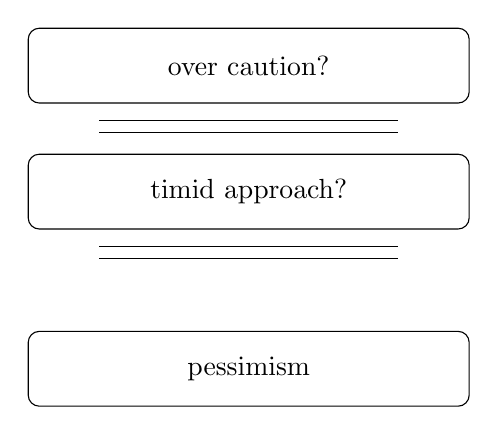
\begin{tikzpicture}
\node[draw, rounded corners, align=center, minimum width=5.6cm, minimum height=0.95cm] at (0,2.4) {over caution?};
\draw (-1.9,1.7) -- (1.9,1.7);
\draw (-1.9,1.55) -- (1.9,1.55);
\node[draw, rounded corners, align=center, minimum width=5.6cm, minimum height=0.95cm] at (0,0.8) {timid approach?};
\draw (-1.9,0.1) -- (1.9,0.1);
\draw (-1.9,-0.05) -- (1.9,-0.05);
\node[draw, rounded corners, align=center, minimum width=5.6cm, minimum height=0.95cm] at (0,-1.45) {pessimism};
\end{tikzpicture}
\caption{Cautious vertical reconstruction of the chalkboard stack. The question marks indicate transcript-assisted completions, and the horizontal marks are treated as separators rather than equal signs.}
\end{figure}

\begin{remark}
The reconstruction is intentionally conservative. It preserves the board's vertical logic without claiming that the chalk contained a formal chain of equalities.
\end{remark}

\subsection{Question \& Answer}

Here the lecture pauses for its cleanest explicit puzzle.

\paragraph{Question.} Why should the same measure affect two people in two different ways?

\paragraph{Answer.} Because the measure is fixed, but the reading is not.

\begin{align}
m &= \tfrac12,\\
m &\mapsto \text{``half empty''},\\
m &\mapsto \text{``half full''}.
\end{align}

That example matters because it gives the lecture a worked model. The object does not change. The interpretation changes. The conclusion then follows with precision: our lives are affected not only by how things are, but by how we think they are. Pessimism is therefore a disciplined misreading.

\section{The Mental Factory, Guarded Inputs, And The Last Disease}

Once the half-glass puzzle has been answered, the lecture broadens again. It is not enough to say that interpretation matters; we now ask what forms interpretation. The answer is the mental factory. Thought is treated as ingredient, and life as the fabric built from those ingredients.

\begin{definition}
The \emph{mental factory} is the process by which repeated thought becomes the economic, social, and financial fabric of a life.
\end{definition}

\begin{align}
\text{thoughts} &\rightarrow \text{ingredients},\\
\text{ingredients} &\rightarrow \text{economic/social/financial fabric}.
\end{align}

The virtue of this model is that it gives us a mechanism. Once thought is ingredient, the lecture can immediately ask about quality control. What are we reading? What are we taking in? What are we allowing to be dumped into the factory?

The talk to the students in Danbury sharpens this into a simple recipe:
\begin{enumerate}
\item select the right ingredients,
\item keep out the wrong ingredients,
\item remember that everything starts with thought.
\end{enumerate}

The coffee example then becomes an explicit worked instance.

\begin{align}
\text{sugar in coffee} &\Rightarrow \text{safe},\\
\text{strychnine in coffee} &\Rightarrow \text{dead}.
\end{align}

The logical point is not chemistry but source-indifference. It does not matter who puts the wrong ingredient into the cup. The effect remains destructive. Hence the practical injunction: stand guard at the door of the mind.

Only after this mechanism has been established does the lecture name its final disease, complaining or murmuring. That order is important. Complaining is not merely bad manners. It is bad input, repeated and normalized, until it begins to reshape the future.

\begin{equation}
5\ \text{minutes of complaining} \Rightarrow 5\ \text{minutes wasted}.
\end{equation}

The children of Israel are then used as the last worked example. Delivered from slavery, they nevertheless do not reach the promised land because complaint becomes their settled mode of response. The lecture's closing inference is therefore severe but consistent: indulge this disease long enough, and the future is canceled.

\section{Summary}

The lecture begins by classifying the negative and ends by disciplining the mind. Negative conditions are normal, but they are not to be enthroned. Because the world has defaults, inactivity yields darkness, drift, and loss. Because attitude has diseases, they must be named rather than sentimentalized. Because interpretation governs effect, pessimism is not harmless description but active misreading. And because thought becomes ingredient, the mind must be guarded if the fabric of life is to be built well. We end, then, where the lecture itself ends: the war is on, and the practical task is to keep the good we begin from being undone by drift, bad input, and complaint.